\begin{document}
\begin{frame}{Main Research Focus}
    \begin{itemize}
        \item Can Generative Adversarial Networks (GANs) improve low-light underwater images?
        \item  FishSense cameras often capture noisy, low-light images that hinder analysis.
        \item Goal: Propose and implement a GAN-based pipeline to enhance visual clarity and usable data.
    \end{itemize}
\end{frame}

\begin{frame}{Why Use GANs for FishSense?}
    \begin{itemize}
        \item FishSense images are often captured in low-light, underwater environments
        \item Traditional image processing struggles with noise and low contrast
        \item GANs are known to perform well in denoising and super-resolution tasks
        \item We aim to adapt GANs to improve underwater visual quality,
    \end{itemize}
\end{frame}

\begin{frame}{Proposed Methodology}
Based on two papers I read:
    \begin{enumerate}
        \item Region-based segmentation of underwater images
        \item Conditional GAN without random noise vector
        \item Use image superimposition: overlay multiple versions of the same scene with variations in noise, brightness, or angle
        \item Compare original vs processed image quality using SNR and visual quality metrics: SNR and Visual Quality
    \end{enumerate}
\end{frame}

\begin{frame}{Implementation Plan}
    \begin{itemize}
        \item Review relevant GAN architectures and training procedures
        \item Design and prototype in Python using PyTorch or TensorFlow
        \item Train model on collected FishSense dataset
        \item Evaluate outputs against baseline and write final paper
    \end{itemize}
\end{frame}
\begin{frame}{Additional Work: Data Collection}
    \begin{itemize}
        \item Participated in field data collection with FishSense and FishTechy
        \item Used cameras on a research boat to capture real-world training data.
    \end{itemize}

    \vspace{1em}
    \centering
    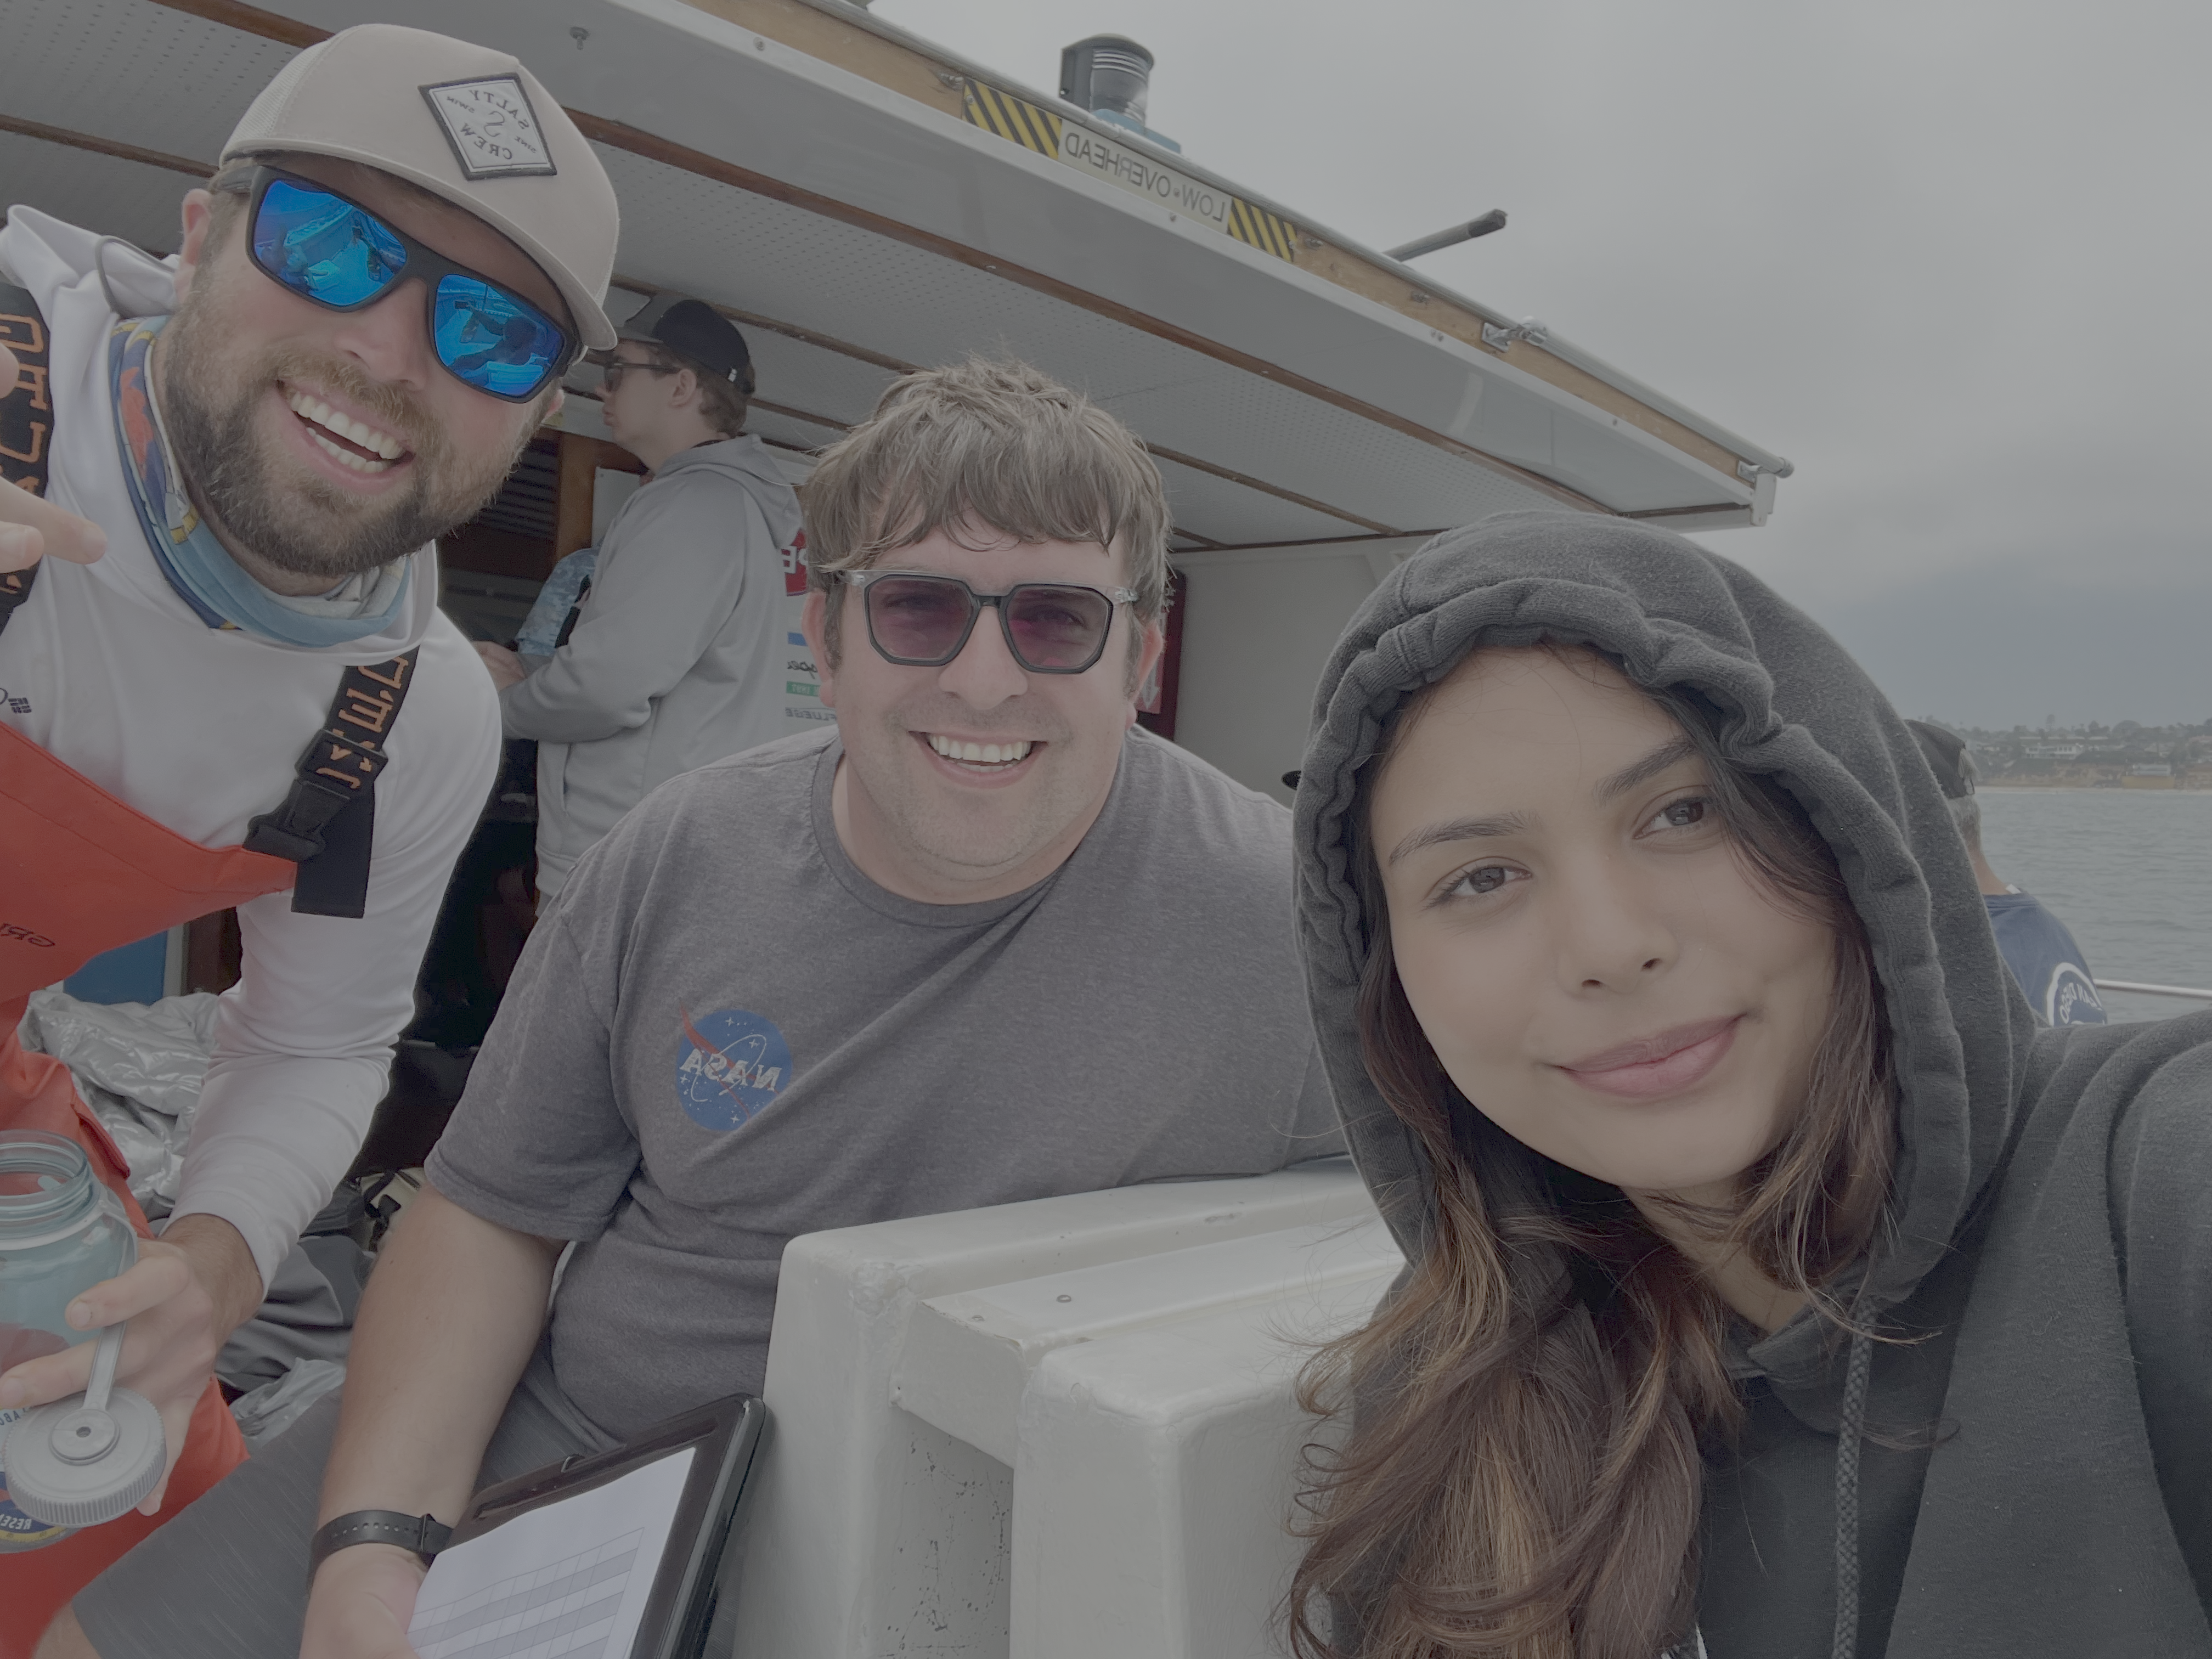
\includegraphics[width=0.7\textwidth, keepaspectratio]{images/fieldop.png}
\end{frame}
    \end{itemize}
\end{frame}

